%% 
%% Copyright 2007, 2008, 2009 Elsevier Ltd
%% 
%% This file is part of the 'Elsarticle Bundle'.
%% ---------------------------------------------
%% 
%% It may be distributed under the conditions of the LaTeX Project Public
%% License, either version 1.2 of this license or (at your option) any
%% later version.  The latest version of this license is in
%%    http://www.latex-project.org/lppl.txt
%% and version 1.2 or later is part of all distributions of LaTeX
%% version 1999/12/01 or later.
%% 
%% The list of all files belonging to the 'Elsarticle Bundle' is
%% given in the file `manifest.txt'.
%% 

%% Template article for Elsevier's document class `elsarticle'
%% with numbered style bibliographic references
%% SP 2008/03/01

\documentclass[preprint,12pt]{elsarticle}

%% Use the option review to obtain double line spacing
%% \documentclass[authoryear,preprint,review,12pt]{elsarticle}

%% Use the options 1p,twocolumn; 3p; 3p,twocolumn; 5p; or 5p,twocolumn
%% for a journal layout:
%% \documentclass[final,1p,times]{elsarticle}
%% \documentclass[final,1p,times,twocolumn]{elsarticle}
%% \documentclass[final,3p,times]{elsarticle}
%% \documentclass[final,3p,times,twocolumn]{elsarticle}
%% \documentclass[final,5p,times]{elsarticle}
%% \documentclass[final,5p,times,twocolumn]{elsarticle}

%% For including figures, graphicx.sty has been loaded in
%% elsarticle.cls. If you prefer to use the old commands
%% please give \usepackage{epsfig}

%% The amssymb package provides various useful mathematical symbols
\usepackage{amssymb}
\usepackage{booktabs}
\usepackage{algorithm}
\usepackage[noend]{algpseudocode}
\usepackage{algcompatible}
\usepackage{multirow}
\usepackage{amsmath}
\usepackage{algorithm}
\usepackage[noend]{algpseudocode}
\usepackage{algcompatible}
%% The amsthm package provides extended theorem environments
%% \usepackage{amsthm}

%% The lineno packages adds line numbers. Start line numbering with
%% \begin{linenumbers}, end it with \end{linenumbers}. Or switch it on
%% for the whole article with \linenumbers.
%% \usepackage{lineno}

\journal{Nuclear Physics B}

\begin{document}

\begin{frontmatter}

%% Title, authors and addresses

%% use the tnoteref command within \title for footnotes;
%% use the tnotetext command for theassociated footnote;
%% use the fnref command within \author or \address for footnotes;
%% use the fntext command for theassociated footnote;
%% use the corref command within \author for corresponding author footnotes;
%% use the cortext command for theassociated footnote;
%% use the ead command for the email address,
%% and the form \ead[url] for the home page:
%% \title{Title\tnoteref{label1}}
%% \tnotetext[label1]{}
%% \author{Name\corref{cor1}\fnref{label2}}
%% \ead{email address}
%% \ead[url]{home page}
%% \fntext[label2]{}
%% \cortext[cor1]{}
%% \address{Address\fnref{label3}}
%% \fntext[label3]{}

\title{Switching Optimisation in Huffman Code for Power Efficient   Data Transmission }

%% use optional labels to link authors explicitly to addresses:
%% \author[label1,label2]{}
%% \address[label1]{}
%% \address[label2]{}

\author{}

\address{}

\begin{abstract}

Reliability of low powered devices is highly dependent on their power efficiency. In digital communication, a significant amount of power is dissipated in data transmission. Different technologies have been emerged to address the issues of power consumption. In CMOS technology, dynamic power accounts for 70\%-90\% of the total power dissipation and it depends on the representation of the data  and increases linearly with switching activities (transition from logic level High to Low and vice versa). Therefore, an efficient representation of data can minimise power consumption by reducing switching activities.  In this paper, we have extended the Huffman code, a widely used data compression technique, by using genetic algorithm to reduce switching activities in the transmitted message. %In Recently the power consumption identified as one of the most pressing challenges of data transmission. Though a considerable reduction of size of data is obtained by Huffman code and several methods have been proposed to improve the data compression rate. These methods improves only the total number of bits without consideration of transmission cost. In this paper, we propose a new approach to reduce the power consumption, by applying genetic algorithm for minimising the total number of switches, either inter- or intra-switch. 
The main objective of the proposed approach is to minimise the switching activities in the codeword of each symbol as well as the switching activities between the symbols.  The approach starts its operation by generating an initial population, a set of Huffman trees, for all the input symbols. Afterwards, the genetic operators such as selection, crossover and mutation are applied to the initial population to improve the quality of the solutions. %The amount of power consumption is proportional to the total number of switches on the whole sequence. 
The performance of the approach is evaluated by applying it to a set of real biological datasets. The experiments yield that the proposed approach reduces the switching activity by $45.47\%$ in the best case, by $36.33\%$ in the average case and by $16.42\%$ in the worst case. 
\end{abstract}

\begin{keyword}
%% keywords here, in the form: keyword \sep keyword

%% PACS codes here, in the form: \PACS code \sep code

%% MSC codes here, in the form: \MSC code \sep code
%% or \MSC[2008] code \sep code (2000 is the default)

\end{keyword}

\end{frontmatter}

%% \linenumbers

%% main text
\section{Introduction}
In the recent years, application of battery-powered portable devices, e.g., laptop computers, personal digital assistant (PDA),  and mobile phones has increased significantly. The reliability and performance of such devices are primarily dependent  on their power consumption, i.e., effective battery life. Bigger battery size could help to improve power efficiency, however, in a portable device the size of the battery is restricted by the size and weight of the device itself. The cost of providing power to both portable and non-portable devices has resulted in significant interest in power reduction. CMOS technologies were developed in order to reduce the power consumption both in data processing and transmission. In \cite{chandrakasan1995}, an approach was proposed to minimise power consumption in CMOS circuits. The method considers optimising the technology used to implement the digital circuits, circuits style and topology, the architecture for implementing the circuits and the algorithms that are being implemented in the devices.

As data transmission is a common operation in both portable and non-portable devices, therefore, reducing power dissipation in transmission systems is important. Authors in \cite{Gregori2004,Yates04} have investigated different criteria for low power data transmission. Power consumption for data transmission in IEEE 802.11 multi-hop networks and 3G mobile wireless networks were analysed in \cite{Le11} and \cite{toorisaka12} respectively.  In order to increase transmission speed and reduce power dissipation, parallel data transmission methods are widely used. However, parallel transmission is limited to short distance communications, e.g. locally connected devices, internal buses. Ruling out the possible availability of parallel transmission links over long distance, we are left with its serial alternative only. If we attempt to transfer big files, e.g. DNA sequences, over a serial transmission link then it would take a significant amount of time and obviously a significant amount power would be dissipated in the process. However, data compression techniques are widely used to reduce size of data before transmitting over serial medium to reduce transmission time and cost.

Huffman code \cite{Huff51} is an entropy
encoding algorithm widely used for lossless data compression. For any given set of symbols and associated occurrence probabilities, Huffman algorithm generates a binary tree (Huffman tree) to encode a message with an optimal number bits. The codeword for a distinct symbol is generated by traversing the tree from the root to
the leaf node representing the symbol. In this traversal process, a move towards a left and a right node is represented by $0$ and $1$ respectively. A major drawback of the classical Huffman code is that the whole stream must be read prior to encoding. To transmit a binary string, power dissipation  is proportional to the number of switching, i.e., transition from $0$ to $1$ and vice versa, present in a transmitted string. Although a number of approaches like \cite{Gol12,Kab14} have extended the classical Huffman code by treating binary bits differently (with unequal letter cost), a little effort has been made to optimise the switching activities in the Huffman code to develop a power efficient Huffman code. To the knowledge of the authors, the only effort to generate Huffman code considering switching activity is seen in \cite{Chen06}. This approach follows a greedy strategy and works in two steps to reduce total number of switching in the Huffman code. In the first step the switching activity between each pair of symbol (inter-switch) is reduced and then in the second step switching activity in the codeword for each each symbol (intra-switch) is reduced. As the optimisation is done independently in two steps therefore it is highly likely that the gain obtained in the first step may be compromised in the second step and vice versa. 

In this paper, a genetic algorithm based approach is proposed to reduce the total number of switching where inter-switch and intra-switch is optimised in a single step, i.e, a balance is made between the two different types of switching. The approach generates a set of trees, each one represents a set of codewords (solution). After that a set of genetic operators such as selection, crossover and mutation is used to evolute (create new trees) the population to minimise number of total switches. The evolution process is controlled by the total number of inter- and intra-switches.  Inter-Switch between two adjacent symbols depend on the their codewords, i.e., how the codeword of the preceding symbol finished (with $0$ or $1$) and how the codeword for the descendent symbol started. If the end bit of the preceding symbol and the staring bit of the successor symbol differs then their exists a switch and the total number of switch is the number of times the two symbols in consideration occurs one after another. To obtain the total number Inter-Switch between pair of symbols, we used a descendent matrix which is a two dimensional matrix represents the number of occurrence of each symbol after another. This matrix is formed when the message to be transmitted is scanned to obtain the frequency of distinct symbols. The number of intra-switch for a symbol is calculated by multiplying the frequency of that symbol by the number of logic level transition ($0$ to $1$ or $1$ to $0$) in the codeword of the symbol. The efficiency of the approach is evaluated by applying it to a set of biological datasets. The experiments yield that the proposed approach improves the total number of switches by $X\%$ in the best case, by $Y\%$ in the average case and by $Z\%$
in the worst case.

The rest of the paper is organised as follows:
Section 2 presents the background study of the
relationship of switching activity with power consumption, the relation of switching with Huffman code and the issues in biological data transmission. The proposed approach is described in Section 3. Experimental results and
discussion are presented in Section 4 . Finally,
concluding remarks are presented in Section 5. 
\section{Background}
\subsection{Effect of Switching in Power Consumption}
CMOS is the most widely used technology implemented in VLSI chips because of their power efficiency. Power dissipation in CMOS circuits has three different components: dynamic, static, and leakage \cite{Weste88}.
\begin{equation*}
P_{avg} = P_{dynamic}+P_{static}+P_{leakge} ~~~~~~~~~~~~~~~~~~~~~~~~~~~~~~~~~~~~~~
\end{equation*}
\begin{equation}
~~~~~~~~~~~~= 0.5 \times C_{L} \times V_{dd}^{2}\times E(sw)\times f_{clk} + I_{sc} \times V_{dd}+I_{leakage} \times V_{dd}
 \end{equation}
 where\\
  $P_{avg}$ is the average power dissipation
  $C_{L}$ is the load capacitance, \\
  $V_{dd}$ is power supply,\\
  $E(sw)$ is average transition (switching) number per clock cycle ,\\
  $f_{clk}$ is the clock frequency,\\
  $ I_{sc}$ is the short circuit current, and\\
  $ I_{leakage}$ is the leakage current.\\
Out of the three components, the dynamic power dissipation is the dominant and it counts for 70\%-90\% of the total power consumption\cite{pedram1996}. Therefore, optimisation of dynamic power consumption is considered in this paper. In CMOS circuit, dynamic power consumption arises when the load capacitance ($C_{L}$) is charged to address a transition from low to the high voltage level.  The parameters $C_{L}$, $V_{dd}$, and $f_{clk}$ in dynamic power dissipation are primarily determined by the circuit layout and the fabrication technology. However, amount of switching, $E(sw)$ completely depends on the digital representation of the data. As the dynamic power dissipation is proportional  to the average number of switching, thus a reduction in the total switching number will eventually results in the reduction of the dynamic power consumption. Therefore, we focus on reducing total amount of switching in Huffman code to improve power efficiency of digital data processing.
%In this paper, by switching we mean a transition from `0' to `1' or `1' to `0' in a binary sequence. 
\subsection{Huffman Code and Its Relationship with Switching Activity}
%\subsubsection{Relationship between switching and Huffman Code}
In computer science and information theory, Huffman code is an entropy encoding algorithm used for lossless data compression. The classical Huffman code requires to pass the input data two times to complete the encoding operation. In the first pass, it reads the whole stream to determine the occurrence frequencies of distinct symbols. After that, symbols along with their frequencies are used to generate a binary tree known as Huffman tree. The process of Huffman tree generation is shown in algorithm 1 \cite{Cormen2001}.
 
\begin{algorithm}[!thpb]
\label{alg1}
\caption{Huffman(C)}
\begin{algorithmic}[1]
\State $n \leftarrow |C|$
\State $Q \leftarrow C$
\FOR {$i = 1~to~n-1$}
\State $allocate~a~new~node~z$
\State $left[z]$ $\leftarrow$ $x$ $\leftarrow$ $EXTRACT\_MIN (Q)$
\State $right[z]$ $\leftarrow$ $y$ $\leftarrow$ $EXTRACT\_MIN (Q)$
\State $f[z]$ $\leftarrow$ $f[x] + f[y]$
\State $INSERT (Q~,~z)$
\ENDFOR
\State \textbf{$retur$n} $EXTRACT\_MIN (Q)$
\end{algorithmic}
\end{algorithm}
In the algorithm, C is the set of n distinct symbols, and each symbol $ c\in C$ has a frequency denoted as f[c]. The algorithm starts its operation with a set of $|C|$  leaf nodes where each node corresponds to a distinct symbol. After that, a sequence of $|C|-1$ merging operation is performed to obtain the final tree. The merging is done by extracting two least frequent symbols from the minimum priority queue, $Q$, and creating and inserting a new node (parent) to the queue for that two symbols. These two symbols are considered as the left and right child of their parent node respectively. The frequency of the new  node is calculated as the sum of the frequency of its child nodes.  The resultant tree ensures the optimal encoding of symbols to obtain maximal compression performance. %The tree is traversed from the root to the leaf nodes to obtain the unique codeword (binary string) for different symbols. 
To form a codeword for a symbol, the tree is traversed from the  root to the leaf node representing the symbol. In the traversal process, any move made towards the left direction is replaced by `0' and any move towards the right direction is replaced by `1'. As a result codeword for each symbol consist of a sequence of 0's and/or 1's. Once the codewords are obtained, in the second pass, the Huffman algorithm encodes the symbols of the input message with the codewords, thus reduce the size of the whole message.
For a set of symbols more than one Huffman tree is possible, i.e., optimal solution can be obtained from different structure of the tree. As the codeword of a symbol depend on its position in the tree, therefore changing the structure of the tree will change the codeword for the symbol. A codeword can contain zero or more switching activity within itself refereed to as intra-switch. For example, if a symbol `A' is assigned a codewrod `000' then there is no intra-switch, on the other hand, if the codeword `101' is assigned to a symbol `B` then their exist two intra-switches. When the codewords of different symbols are concatenated together during transmission they form switching based on the head and tail bit of the codewords. For example, if we want to transmit `AB' then according to the above codewords we will transmit `00\textbf{01}01' which will result in an inter-switch because the tail bit (0) of `A' and the head bit (1) of `B' are different. That means, in this case, we have three total switches--two intra-switches and one inter-switch. Now if `B' is assigned the codeword `010', the new transmitted string is `00\textbf{00}10', then we still have two intra-switches for the codeword of `B' but the inter-switch no more exists. So, changing tree structure, i.e., codewords, will change the total number of switching. Hence, the aim of this paper is to find an optimal Huffman tree that will minimise the total number of switching by making a balance between intra- and inter-switches.

\subsection{Issues in Biological data transmission}
The size of biological databases are continuously increasing. In the last decade the access to these databases has increased significantly. The exponential growth of these databases pose a big problem to all biological data processing methods~\cite{Doug08}. Data compression methods are widely used to reduce the overheads of treating, e.g., transmitting, the high volume of data. The main objective of data compression methods is minimising the number of bits in the data representation. Authors in~\cite{bra09} proposed a new approach to genomic data compression based in suffix and common substring and code the difference with Huffman code. In~\cite{chr09}, authors propose a general scheme based on Huffman code for coding only the difference between the target genome and the referential one. Recently, a method has been proposed to deal with the transmission of genomic data as an email attachment~\cite{wan11}. All the methods used for biological data compression aims only at reducing the size of the data. However, due to the huge size of the input data, the compressed data contains a huge number of switching in them which has a big impact on power consumption. As no consideration is paid to the reduction of switching, hence, the compression process may be size efficient but not power efficient. Therefore, it is believed that a more efficient compression of biological data can be obtained by optimising the size of the data as well as the total number of switching in the transmitted data. %Cost of data transmission is based on two point, firstly the size of the data which has been improved considerably in the recent year with the improvement of Huffman code. Secondly, is the number of switches on the generated codes. %The power consumption increase linear with the number of switches.
\section{The proposed approach for Switching Optimisation}
The main objective of the approach is to minimise the total number of switching in the representation of data produced by the Huffman algorithm. To do so, it is required to minimise both intra- and inter-switches among the codewords. The total number of intra-switch depends on the codewords themselves and the frequency of the symbols. As a result, for  a given set of codewords an optimal number of intra-switches can be obtained by assigning the most frequent symbol with the codewords with minimum number of switching. However, it will not ensure the optimal number of inter-switches. Because, inter-switches not only depend on the codewords of the symbols but also the association between the symbols. By association, we mean how many times a symbol occurs after another symbol in the whole message, i.e., all possible pairing combination among the symbols. As the number of distinct symbols increases in the message the number of combination increases. So improving total number of inter-switching is a combinatorial problem.

Genetic algorithm (GA) has widely been applied to solve a range of combinatorial problem in complex VLSI design~\cite{chan1991macro,bright1996genetic,cohoon1987genetic}. For this reason, the GA is identified as a potential solution to the above mentioned problem. GA is one the of the most popular bio-inspired meta-heuristic algorithm inspired by the natural evolution of species~\cite{gen1}. It is a population based algorithm starts with the generation of a random initial population. The population contain a set of feasible solutions called individuals, that are usually far from the optimal. The GA optimisation process uses a set of natural genetic operators such as selection, crossover and mutation to converge to the optimal solution.
\subsection{ Data preparation and population generation}
A genome is an expansion of DNA sequence which is a set of nucleotides that encodes a protein. These nucleotides are bounded together and each order define a specific protein. Three nucleotides form a triplet and interpreted as a specific amino acid ~\cite{Harvey00}. For this reason, the whole sequence is divided into a set of triplets.  As each DNA sequence contains a combination of four nucleobases\textemdash guanine (G), adenine (A), thymine (T), and cytosine (C), therefore we will have $4^3=64$ possible triplets. As mentioned earlier that the classical Huffman code requires reading the whole sequence prior to encoding. So, in this case, the whole DNA sequence is read considering different triplets as distinct symbols. Frequencies for each of the triplets are calculated and  the adjacency matrix (a symmetric 2D matrix) is also created which represents how many times a triplet occurs after each of the other triplets.  After that, a random set of Huffman trees are generated for the input symbols (triplets) which are considered as the initial population for the GA.
 \subsection{Genetic operations}
\subsubsection{Selection}
The first operator of the genetic algorithm is the selection. The main objective of the selection is to choose the part of the current  population to be a candidate for the different genetic operators in order to breed the next generation population. Many selection techniques have been proposed in the literature~\cite{bli95}. In this approach the  process of natural selection is maintained. First we generate a random pair numbers \textit{$rand$} between 2 and the population size, this number represent how many parents will be processed. After that, an unbiased random selection of \textit{$rand$}~individuals (solutions) from the population is maid. 
\subsubsection{Crossover}
The main operator of the GA is the crossover, allows to construct new solutions from the selected part of the population~\cite{osa14}. The selected solutions are ranked by fitness and crossover two by two from high fitness to low. The main objective of the crossover is to benefits from the two good solutions in order to generate a better solution. An internal node for each tree (solution) is selected (\textit{$node1$},\textit{$node2$}), these two nodes must have the same number of leaf nodes (contain the same number of codes). The crossover operation will create two new trees (solutions), the first child (second) contain the nodes that are not children of the \textit{$node1$} (\textit{$node2$}) and we replace the children of \textit{$node1$} (\textit{$node2$}) by the children of \textit{$node2$} (\textit{$node1$}) (see fig.1). 
\subsubsection{Mutation}
The mutation operator changes the positions of two leaf nodes of the generated children (result of the crossover)~\cite{muhlenbein1992genetic}; this introduce the diversity in the search process, this diversification strategy allow the algorithm do conference to the global optimum. The algorithm for this operator goes through the leaf nodes and change the position of two leaf nodes from a parent to another and selects the ones to change according to a fixed mutation rate (see fig.1).
\subsection{Population update}
The crossover operation aims to generate new solutions from the current solution to built the second generation of the population. Furthermore, the mutation provide the diversity on the search space solution by changing the position of  nodes on the same tree. After these two operations, the next step of the genetic algorithm is two to breed the new population (see fig.2). Firstly the new solutions (children) are added to the current population, after that the population is ranked by fitness. The algorithm remove the worst solutions until the initial size of the population is achieved. The algorithm genetic repeat these operators until the stopped criteria is achieved, in this algorithm the stopped criteria is when the objective function (number of switches) stop decreasing.
\begin{algorithm}[!btph]
\caption{Switches optimising Huffman codes}
\label{alg1}
\begin{algorithmic}[1]
\REQUIRE Textual representation of a Genome
\ENSURE Low switches Huffman codes
\STATE Generate triplet frequencies and adjacent matrix 
\STATE Generate the initial  population of trees
\REPEAT 
\STATE Select part of the population
\STATE Generate children candidates via crossover
\STATE Mutate children
\STATE Add children to population
\STATE Rank by fitness
\STATE Remove worst solutions until population limit
\UNTIL{The switches number stop decreasing}
%\algstore{myalg}
\end{algorithmic}
\end{algorithm}
\begin{figure}[tbph]
\begin{center}
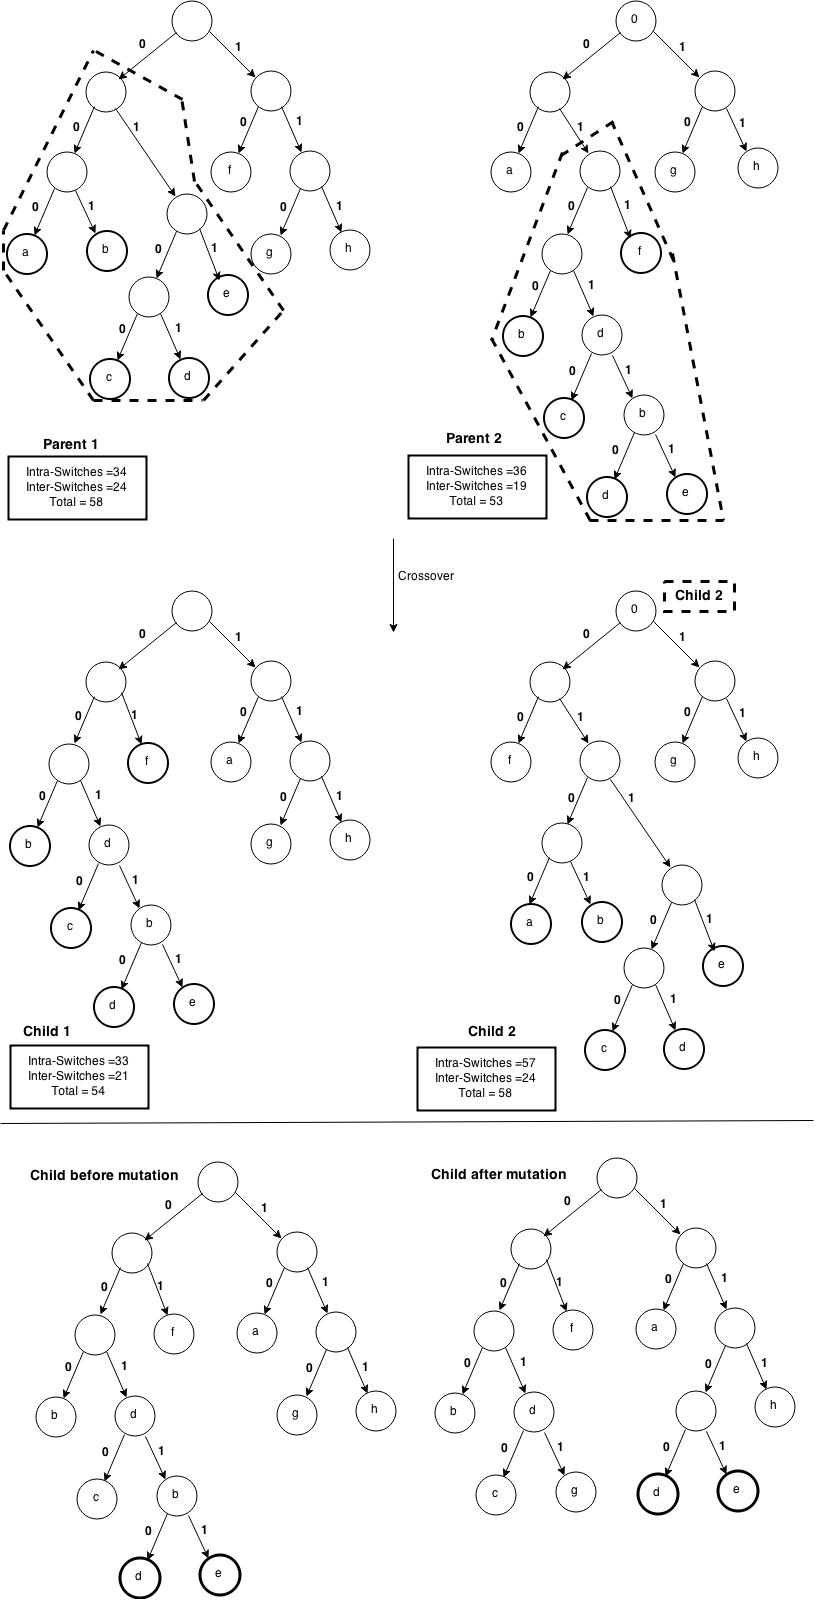
\includegraphics[width=400pt,height=545pt]{Images/Drawing1-1.jpg}
\caption{The Crossover operator}
\end{center}
\label{Fig1}
\end{figure}
\begin{figure}[tbph]
\begin{center}
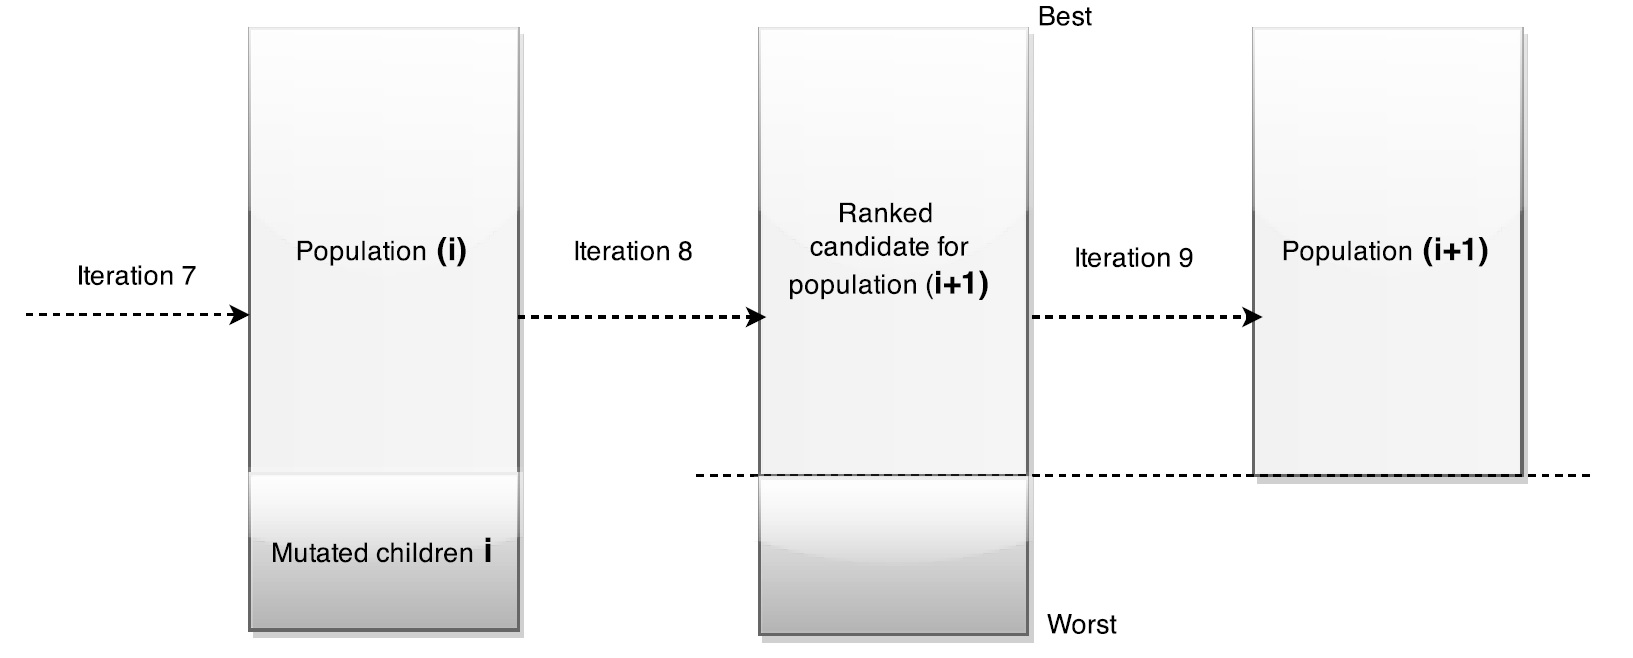
\includegraphics[width=350pt,height=170pt]{Images/Drawing3.jpg}
\caption{Population update for genetic algorithm}
\end{center}
\label{Fig2}
\end{figure}


\section{Experiments and Comparison}
The approach has been evaluated with different real genomic biological data. Different genomes size have been used for the evaluation, from small genome to human chromosome in order to evaluate the efficiency of the approach.The datasets were downloaded as FASTA text file from a recent version of The National Center for Biotechnology Information (NCBI) available on $(http://www.ncbi.nlm.nih.gov)$ \cite{pruitt2009ncbi}. The used genomes are described in table 1, the size are given in Megabyte and the reference on the NCBI database.

\begin{table}[!thpb]

\small
\label{table3}
\caption{Datasets description}
%\begin{center}
\centering
\begin{tabular}{c  c  c c}
\toprule
$\textbf{Data sets}$ &$\textbf{Name}$ &	$\textbf{Size (MB)}$ &	$\textbf{Reference}$ \\\hline
Genome 1& Mycobacterium smegmatis &  6.66 & CP009496  \\\hline

Genome 2& Amycolatopsis benzoatilytica & 8.30 & NZ\_KB912942 \\\hline

\multirow{2}{*}{Genome 3}&Mycobacterium rhodesiae& \multirow{2}{*}{6.11} & \multirow{2} {*}{CP003169}\\ 
&NBB3& &\\
\hline

\multirow{2}{*}{Genome 4 }&Streptomyces bottropensis& \multirow{2}{*}{8.54} &
\multirow{2}{*}{NZ\_KB911581} \\ 
& ATCC 25435 \\
\hline
    
\multirow{2}{*}{Genome 5}&Mycobacterium smegmatis& \multirow{2}{*}{ 6.66} &\multirow{2}{*}{CP009494             } \\ 
&str. MC2 155 \\
\hline

\multirow{2}{*}{Genome 6}&Mycobacterium smegmatis& \multirow{2}{*}{6.76} &\multirow{2}{*}{NZ\_KI421511}\\   &MKD8& &\\
\hline
    
Genome 7& Bradyrhizobium WSM471&  7.42 &NZ\_CM001442\\\hline

\multirow{2}{*}{Genome 8}&Amycolatopsis thermoflava&  \multirow{2}{*}{8.27} &\multirow{2}{*}{NZ\_CM001442}\\   &N1165 & \\
\hline

\multirow{2}{*}{Genome 9}&Bacillus thuringiensis&   \multirow{2}{*}{5.74} &\multirow{2}{*}{ NZ\_CM000747 }\\    &Bt407&\\
\hline    

\multirow{2}{*}{Genome 10}&Bacillus thuringiensis& \multirow{2}{*}{6.03} &\multirow{2}{*}{ NZ\_CM000748}\\    &serovar thuringiensis& \\
\hline
    
\multirow{2}{*}{Genome 11}&Pseudomonas aeruginosa& \multirow{2}{*}{6.48} &\multirow{2}{*}{NZ\_AFXI01000001}\\    &9BR&\\
\hline
    
\multirow{2}{*}{Genome 12}&Bacillus thuringiensis&  \multirow{2}{*}{5.97} &\multirow{2}{*}{ NZ\_CM000753}\\    &serovar berliner ATCC &\\
\hline
    
\multirow{2}{*}{Genome 13}&Bacillus thuringiensis& \multirow{2}{*}{5.75} &\multirow{2}{*}{ NZ\_CM000750 }\\    &serovar pakistani&\\
\hline
    
\multirow{2}{*}{Genome 14}&Pseudomonas aeruginosa& \multirow{2}{*}{6.28} &\multirow{2}{*}{CP006982}\\    &LES400&\\
\hline

\multirow{2}{*}{Genome 15}& Mus musculus & \multirow{2}{*}{25.58} &\multirow{2}{*}{GL456087}\\  &chromosome 1&\\
\hline

\multirow{2}{*}{Genome 16}& Danio rerio & \multirow{2}{*}{56.14} &\multirow{2}{*}{CM002885}\\ & chromosome 1 &\\
\hline
\multirow{2}{*}{Genome 17}&Homo sapiens & \multirow{2}{*}{76.64 } &\multirow{2}{*}{  CM000680  }\\    & chromosome 18 &\\
\hline
\multirow{2}{*}{Genome 18}&Homo sapiens & \multirow{2}{*}{99.94} &\multirow{2}{*}{CM000684   }\\ & chromosome 22&\\
\hline
%\bottomrule
\end{tabular}
%\end{center}
\end{table} 

\begin{table}[h]
\renewcommand{\arraystretch}{1.1}
\small
\label{table4}
\caption{Comparison of performance among classical Huffman code, CCA, and OCCA without penalty}
%\begin{center}

\begin{tabular}{c  c c  c c  c c}
\hline
 & Huffman Algorithm & P \\\hline
\\\hline
Genome 1& 18.16 & 10.05 & 44.65 \\\hline
Genome 2& 24.66 &  15.63 & 36.61 \\\hline
Genome 3&18.46 &  10.66&  42.25\\\hline
Genome 4&25.18&16.26& 35.42\\\hline
Genome 5& 19.24& 16.08 &16.42 \\\hline
Genome 6& 19.61&14.96&23.71\\\hline
Genome 7& 22.40 &13.21&41.02\\\hline
Genome 8&23.87 & 17.70 &25.84\\\hline
Genome 9&17.66 &10.04&43.14\\\hline
Genome 10& 18.14 &9.89& 45.47 \\\hline
Genome 11&19.63&11.48&41.51 \\\hline
Genome 12& 17.59&11.86&32.57 \\\hline
Genome 13& 17.39&10.93&37.14\\\hline
Genome 14&18.53 &11.64&37.18 \\\hline
Genome 15&78.19 &50.60&35.28 \\\hline
Genome 16& 168.98& 102.13&39.56 \\\hline
Genome 17&217.68 &130.93 & 39.85 \\\hline
Genome 18& 243.70& 149.80&38.53 \\\hline
%\bottomrule
\end{tabular}
%\end{center}
\end{table}
Table 2 presents thee results obtained by the proposed approach and classical Huffman code. The results are presented with the total number of switches and the improvement rate. The results shows that the proposed approach optimise the power consumption of the whole genome by reducing the total number of inter- and intra-switches. In the best case the proposed approach improves power consumption over classical Huffman code by $x$, in the worst case by $x$, and on an average by $x$. The proposed approach optimise the total number of switches by swapping finding the best arrangement of nodes on the codewords tree with the best allocation of these codewords to the different frequencies (triplet). The approach continue swapping between the population individuals until a balance is found between inter-switches and intra-switches.
 
\section{Conclusion}
In this paper, we showed how switching activities affect the power consumption in digital communication. After that, a relationship between the Huffman code and the switching activities is shown. Genetic
algorithm is identified as a potential method to optimise the total number of  switching: inter- and intra-switching in Huffman code.  Subsequently, an approach is proposed to show how the genetic algorithm can be used to reduce the power consumption in biological data transmission by reducing total number of switching in the  transmission. The proposed approach starts its operation by generating a set of feasible solutions (Huffman trees), each one contains a set of codewords for the input symbols. After that, the approach uses a set of natural genetic operators to improve the quality of the solutions by generating new solutions. The evolution of the population is controlled by the total number of switching. The advantage of this approach is that it minimises the total number of switching considerably, thus increases the power efficiency data transmission.   
The effectiveness of the proposed approach is evaluated by applying it to several biological data sets with different sizes varied from small genome to a human chromosome. The performance of the approach has been compared with the performance of the classical Huffman code. The results show that the proposed approach reduces the total number of switching significantly to improve the power efficiency of biological data transmission. %The experiment shows that the proposed approach improves Huffman code in the best case with $best$,  $average$ in the average case, and $worst$ case. 
In the future, we hope to improve the allocation method of codewords to different symbols to reduce further the total number of switching.

%% The Appendices part is started with the command \appendix;
%% appendix sections are then done as normal sections
%% \appendix

%% \section{}
%% \label{}

%% If you have bibdatabase file and want bibtex to generate the
%% bibitems, please use
%%
%%  \bibliographystyle{elsarticle-num} 
%%  \bibliography{<your bibdatabase>}

%% else use the following coding to input the bibitems directly in the
%% TeX file.

\section*{References}
\bibliographystyle{elsarticle-num}
\bibliography{mybib}
\end{document}
\endinput
%%
%% End of file `elsarticle-template-num.tex'.
